\section{Problème, usage et proposition de valeur}

\subsection{Une barrière linguistique qui devient un risque financier}

Comprendre une interface bancaire ne consiste pas seulement à reconnaître des
mots. L’utilisateur doit distinguer une action irréversible d’une étape
préparatoire, un crédit d’un débit, un montant d’un total avec frais et une
information d’une alerte. Une traduction approximative peut donc réduire
l’accessibilité tout en augmentant le risque.

\begin{figure}[H]
\centering
\begin{minipage}[t]{0.48\linewidth}
  \centering
  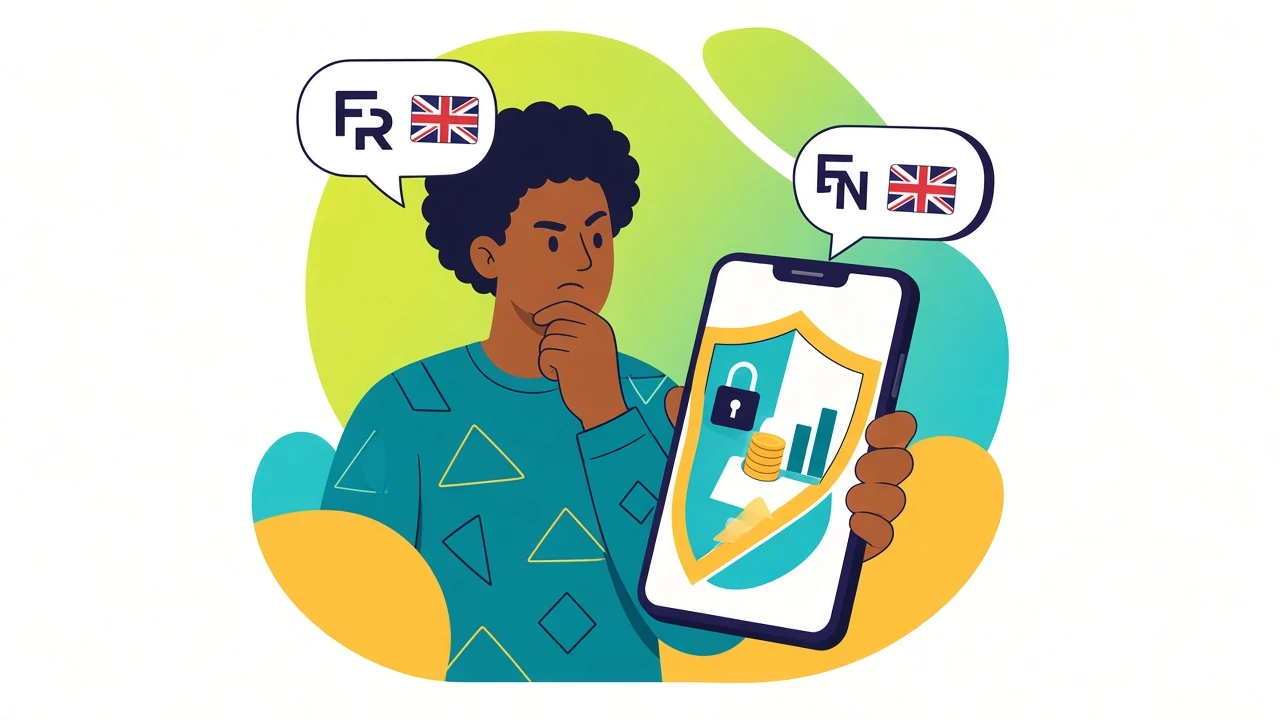
\includegraphics[width=\linewidth]{assets/problem.png}
  \caption*{\textbf{Problème.} Une interface financière uniquement FR/EN peut
  exclure un utilisateur qui comprend mieux une langue nationale.}
\end{minipage}
\hfill
\begin{minipage}[t]{0.48\linewidth}
  \centering
  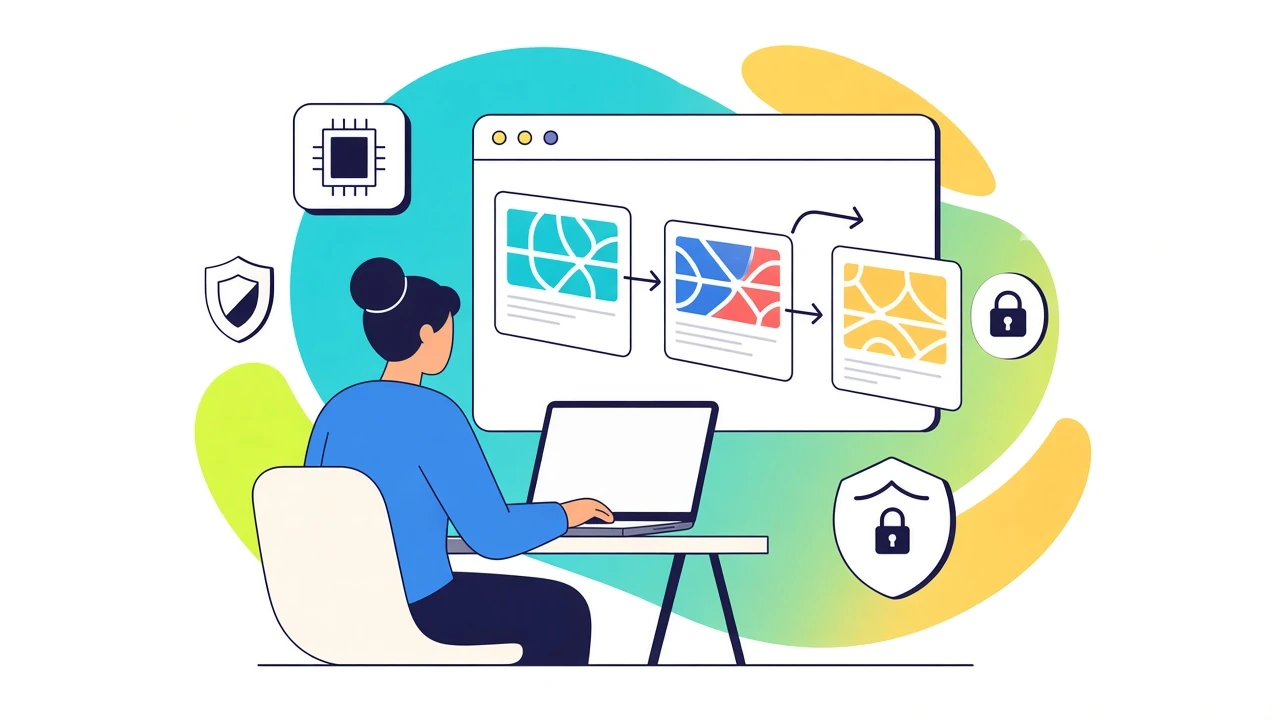
\includegraphics[width=\linewidth]{assets/solution.png}
  \caption*{\textbf{Réponse KORA.} Une couche locale traduit la surface
  accessible tout en isolant les valeurs sensibles.}
\end{minipage}
\end{figure}

KORA se place entre l’utilisateur et la représentation visuelle de la page.
Le service financier continue de calculer les frais, de gérer son formulaire
et de valider son parcours. L’extension ne remplace pas cette logique : elle
traduit uniquement les textes visibles qui passent ses contrôles.

\subsection{Cas d’usage principal}

\begin{enumerate}
  \item Amina ouvre l’interface Safinum en français ou en anglais.
  \item Elle ouvre la popup KORA et choisit \textbf{Fulfulde}.
  \item Le tableau de bord devient compréhensible en \code{fub}; le solde et
        le numéro de compte restent strictement identiques.
  \item Elle choisit une opération et saisit un montant. KORA traduit les
        libellés, mais le site conserve la valeur et calcule les frais.
  \item Elle saisit le nom, le téléphone, le motif et une note. Ces valeurs
        utilisateur ne sont pas traduites.
  \item Elle vérifie le récapitulatif, confirme et retrouve les mêmes valeurs
        sur le reçu puis sur le tableau de bord.
  \item Un message ou un écran ajouté après chargement repasse
        automatiquement dans le même pipeline de traduction.
\end{enumerate}

\begin{keybox}[Promesse utilisateur]
\textbf{Comprendre} l’action dans sa langue; \textbf{vérifier} les valeurs
canoniques sans altération; \textbf{confirmer} seulement lorsque le sens est
couvert. KORA privilégie la sûreté d’une interface partiellement traduite à la
fluidité trompeuse d’une interface entièrement générée.
\end{keybox}

\subsection{Interface et réversibilité}

\begin{figure}[H]
\centering
\begin{minipage}[c]{0.40\linewidth}
  \centering
  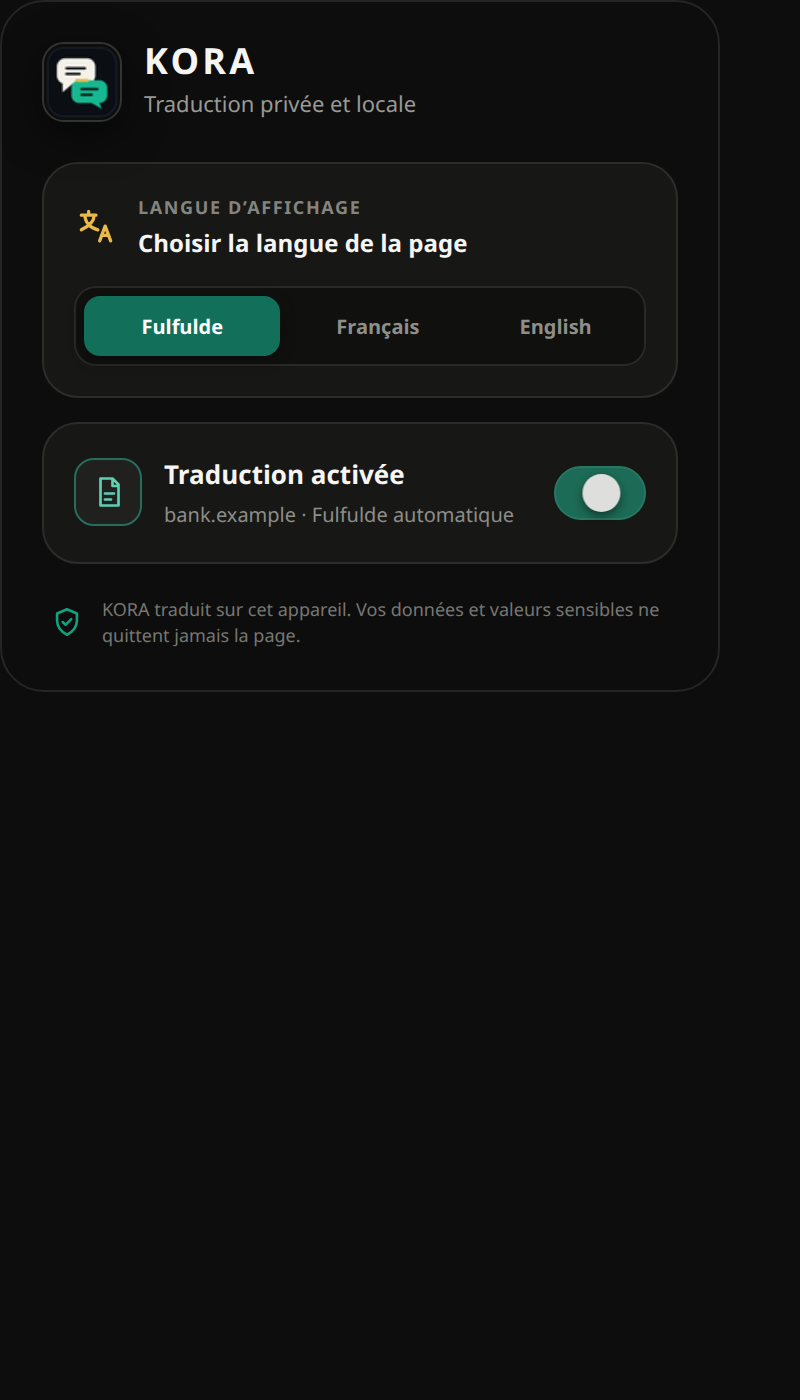
\includegraphics[width=0.72\linewidth]{assets/kora-popup.png}
\end{minipage}
\hfill
\begin{minipage}[c]{0.56\linewidth}
  \textbf{La popup pilote, elle ne traduit pas.}
  \begin{itemize}
    \item \textbf{Fulfulde} active la détection FR/EN et la sortie
          \code{fub}.
    \item \textbf{Français} ou \textbf{English} restaure d’abord les nœuds
          d’origine, puis déclenche le sélecteur natif du site lorsqu’il
          existe.
    \item L’interrupteur suspend ou reprend la traduction sans recharger le
          contenu.
    \item Après une action, la popup se ferme et rend le focus à la page;
          \code{Ctrl+A}, la tabulation et les raccourcis restent natifs.
  \end{itemize}
  \small
  KORA ne fabrique pas une traduction FR$\leftrightarrow$EN : ce changement
  dépend du contrôle linguistique du site. Son propre contrat est
  FR/EN$\rightarrow$\code{fub}.
\end{minipage}
\caption{Popup sombre KORA et comportement des trois choix de langue.}
\end{figure}

\subsection{Parcours financier démontré}

\begin{tikzpicture}[
  node distance=5mm and 4mm,
  journey/.style={draw=Line,fill=Paper,rounded corners=2mm,minimum height=18mm,
    text width=27mm,align=center,font=\small},
  num/.style={circle,fill=Teal,text=white,font=\bfseries,inner sep=2.2pt},
  arrow/.style={-{Latex[length=2.2mm]},thick,color=TealDark}
]
\node[journey] (s1) {\tikz\node[num]{1};\\[1mm]\textbf{Solde}\\compte et historique};
\node[journey,right=of s1] (s2) {\tikz\node[num]{2};\\[1mm]\textbf{Frais}\\type et montant};
\node[journey,right=of s2] (s3) {\tikz\node[num]{3};\\[1mm]\textbf{Bénéficiaire}\\données saisies};
\node[journey,right=of s3] (s4) {\tikz\node[num]{4};\\[1mm]\textbf{Récapitulatif}\\valeurs à vérifier};
\node[journey,right=of s4] (s5) {\tikz\node[num]{5};\\[1mm]\textbf{Confirmation}\\reçu et retour};
\draw[arrow] (s1) -- (s2);
\draw[arrow] (s2) -- (s3);
\draw[arrow] (s3) -- (s4);
\draw[arrow] (s4) -- (s5);
\end{tikzpicture}

Les erreurs \code{AMOUNT\_001}, \code{AMOUNT\_002},
\code{BENEFICIARY\_001}, \code{SECURITY\_001},
\code{SECURITY\_002}, \code{NETWORK\_001} et
\code{CONFIRM\_001} font partie de la matrice de contrôle. Les codes restent
intacts; leurs titres et explications visibles peuvent être traduits.

\subsection{Périmètre observable}

\begin{tabularx}{\linewidth}{@{}Y Y@{}}
\toprule
\textbf{Pris en charge} & \textbf{Hors exposition du navigateur}\\
\midrule
Nœuds texte; boutons; liens; labels; options visibles; \code{placeholder};
\code{aria-label}; \code{title}; contenu ajouté ou remplacé; Shadow DOM
ouvert; iframes autorisées. &
Texte incorporé à une image; pixels d’un \code{canvas}; Shadow DOM fermé;
pages \code{chrome://}; Chrome Web Store; iframe interdite par le navigateur.\\
\bottomrule
\end{tabularx}

Cette frontière est technique et vérifiable : une extension ne peut pas
traduire un texte que Chrome ne lui expose pas sans OCR, contournement ou
permission supplémentaire.
